%
% Chapter 6
%

%% I need to describe muon ID in chaper 4.2 and Tau decay mode finding, tau MVA ID around 4.2 too 
\chapter{LFV event selection}
For both the 8TeV analysis $H\rightarrow e\tau_h$ channel and 13TeV analysis  $H\rightarrow\mu\tau_h$, events are selected in several steps. The loose(base) selection on the different IDs, energy, geometry parameters of the analysis related objects and so on are applied. For both  $H\rightarrow e\tau_h$ and $H\rightarrow\mu\tau_h$ analysis channel, a following cut-based analyses are applied. For $H\rightarrow\mu\tau_h$, a multivariate analysis with Boosted decision tree (BDT) is exploited to provide more sensitive results. 



\section{\texorpdfstring{$H\rightarrow\mu\tau_h$}{Lg}}
\subsection{Loose selection}
In $H\rightarrow\mu\tau_h$ events, tau leptons from signal events decay hadronically and most of the time, $\mu$ candidates pass all the way to the muon detector. SM higgs is much heavier than the LFV decay products $\mu$ and $\tau$, so $\mu$ and $\tau$ are expected to have high $P_{T}$. Since the decay products are boosted, a cut on the $\Delta R>0.3$ is applied, in which $\Delta$R is defined as $\Delta R=\sqrt(\Delta phi^{2}+\Delta eta^{2})$. Higgs particle has no charge, so $\mu$ and $\tau$ candidates are required to have opposite charges. Further, the events with additional $\mu$ and $\tau$ that pass a loose selection, the events with jets that are identified by the combined secondary vertex(CSVv2) b-tagging algorithm \cite{btag_ago} as a b quark jets will be vetoed. The $\mu$ from signal events are boosted and isolated, as mentioned in previous chapter, the trigger HLT\_IsoMu24 or HLT\_IsoTkMu24 is used, the trigger select isolated $\mu$ that have energy higher than 24GeV. An further $P_{T}$ cut on reconstruct $\mu$,  $P_{T}>26$GeV and $|\eta|<2.4$ are applied. $\mu$ are required to pass the recommended Medium $\mu$ ID(chapter 4.2) from CMS collaboration. $\mu$ are required to pass muon ID. For the LHC data 2016, running period BCDEF, ICHEP medium muon ID is applied(table~\ref{tbl:ICHEPMedID}), for running period G and H, also the monte Carlo samples, standard medium muon ID(table~\ref{tbl:standardMedID})are applied to achieve the best performance for muon identification.

Hadronic taus are required to have $P_T>30$GeV,$|\eta|<2.3$, pass old tau decay mode finding(chapter 4.2) and an MVA based tight tau isolation ID(chapter 4.2) and tau discriminators against other objects. These discriminators are very loose MVA based rejection against electrons and the cut-based tight rejection against muons.  


\begin{table}[tpb]
\caption{Muon ID used in the analysis, for the LHC data 2016, running period BCDEF.  \label{tbl:ICHEPMedID}}
\label{tab:antil}
\begin{center}
\begin{tabular}{|l|c|}   
\hline
ICHEP mediumID description                    &  Technical description\\\hline
Loose muon ID                               & PFLoose Muon\\\hline
Fraction of valid tracker hits           & $>0.49$ \\\hline
\multirow{5}{*}{1.Good Global muon}                      &Global muon\\\cline{2-2}
                                                                        &Normalized global-track $\chi^{2}<3$\\\cline{2-2}
                                                                        &Tracker-Standalone position match $< 12$\\\cline{2-2}
                                                                        &kick finder $< 20$ \\\cline{2-2}
                                                                        &Segment compatibility $> 0.303$ \\\hline                                                                       
\hline
2. Tight segment compatibility      & Segment compatibility $>0.451$\\\hline
\end{tabular}
\end{center}
\end{table}


\begin{table}[tpb]
\caption{Muon ID used in the analysis, for the LHC data 2016, running period G and H, also the monte Carlo samples.  \label{tbl:standardMedID}}
\label{tab:antil}
\begin{center}
\begin{tabular}{|l|c|}   
\hline
Standard mediumID description                    &  Technical description\\\hline
Loose muon ID                               & PFLoose Muon\\\hline
Fraction of valid tracker hits           & $>0.8$ \\\hline
\multirow{5}{*}{1.Good Global muon}                      &Global muon\\\cline{2-2}
                                                                        &Normalized global-track $\chi^{2}<3$\\\cline{2-2}
                                                                        &Tracker-Standalone position match $< 12$\\\cline{2-2}
                                                                        &kick finder $< 20$ \\\cline{2-2}
                                                                        &Segment compatibility $> 0.303$ \\\hline                                                                       
\hline
2. Tight segment compatibility      & Segment compatibility $>0.451$\\\hline
\end{tabular}
\end{center}
\end{table}

The events in the analysis are divided into four categories based on the number of jets in the events. In 2-jets categories, it is furthered divided into 2 categories,  2-jet gluon gluon fusion higgs production(ggH) category and 2-jet VBF category based on the value of 2 jets invariant mass($M_{jj}$) . In the 0-jet category, the signal mainly comes from ggH. In 1-jet category, the dominant signal production mode is also ggH, but with a boosted jet associated with the production, some of the VBF higgs signal also shows up in this category. In the 2-jet ggH category, signal evens mainly comes from ggH and in 2-jet VBF, VBF production dominants the production mode.  In the following is a more detailed listing of the selection condition in each categories.

\begin{enumerate}
\item[{\bf 0-jet:}] No events have jets pass the loose PF ID and  with jet $P_T>30$ GeV, $|\eta|<4.7$.
\item[{\bf 1-jet:}] The events with one jet passes losse PF ID and jet $P_T>30$ GeV, $|\eta|<4.7$.
\item [{\bf 2-jets GG:}] The events have two jets pass loose PF ID and with jet $P_T>30$ GeV and $|\eta|<4.7$, also require an invariant mass of the two jets, $\textrm{M}_{jj}<550GeV$. 
\item [{\bf 2 jets VBF:}] The events have two jets pass loose PF ID and with jet $P_T>30$ GeV and $|\eta|<4.7$, also require $\textrm{M}_{jj}>550 GeV$ . 
\end{enumerate} The threshold on $\textrm{M}_{jj}$ has been optimized to give the best expected limits.


\subsection{Cut-based analysis}
With the loose selection, including the categorization, a further cut-based selection strategy is applied. The selected variables that can help distinguish signal from background used in this analysis are the following ones: $P_{T}^{\mu}$, $P_{T}^{\tau}$, $M_{T}(\tau_{h})$. The lepton $P_{T}$ variables are very powerful background discriminant variables, but it will also cause the problem that signal picks under the background. Leptons from signal process  incline to have higher $P_{T}$ values, by cutting tighter on the lepton $P_{T}$, more background events can be removed. However this will also reshape some of the backgrounds, making them peak closer under signal so as making the signal discovery processes affected more by the background statistics fluctuation. In the $H\rightarrow e\tau_h$ analysis, the effect of cutting hard on lepton $P_{T}$ will be shown. So in $H\rightarrow\mu\tau_h$ search, lepton $P_{T}$ variables are kept at loose values and tune on other variables to achieve better signal significance. 

The tuning process is done only with Monte Carlo samples to not double use data. The final results are extract with data, so the double use of data may cause some biases on the results. The fake background estimated with full data driven method, is replaced with the semi data driven estimation in tuning.  
In $M_{T}(\tau_{h})$  channel, the variables tuned are $\textrm{M}_{jj}$ and $M_{T}(\tau_{h})$. The cuts have been optimized to have the most stringent expected limits with the Asimov dataset. If the same cut, but close values of the cut give same expected limits, then chose the loose cut value to have most stringent expected limits and have as much statistics as possible. Examples of obtaining the limits are shown in Fig. \ref{fig:optMT}, the $M_T(\tau_{h})$ for the different categories and Fig.~\ref{fig:optVBFmass}  for the optimization of $\textrm{M}_{jj}$ in 2-jets categories.


\begin{figure}[!htbp]
     \centering
     \subfigure[0 jet]{ 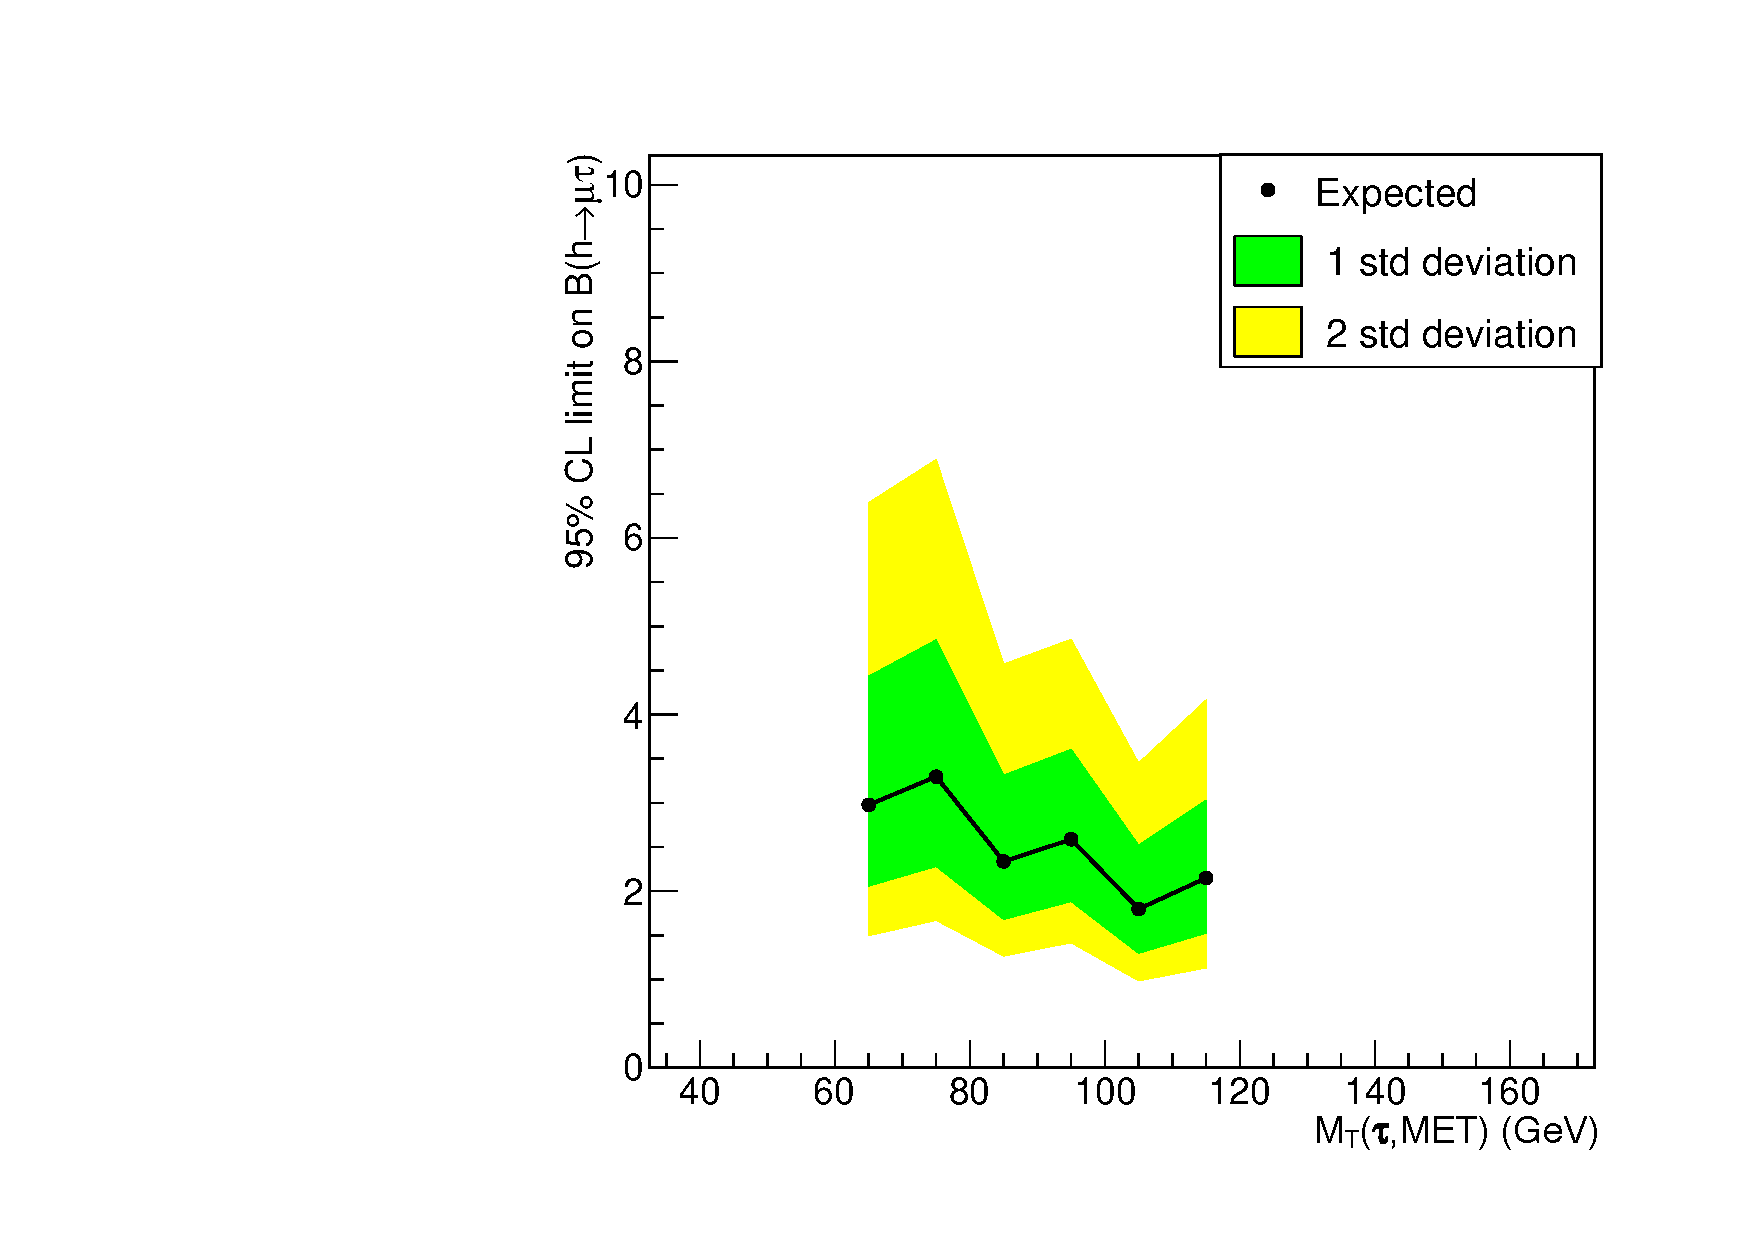
\includegraphics[width=0.4\textwidth]{chapter6/Tuning/ggtMtToPfMet_type1.pdf}}
     \subfigure[1 jet]{ 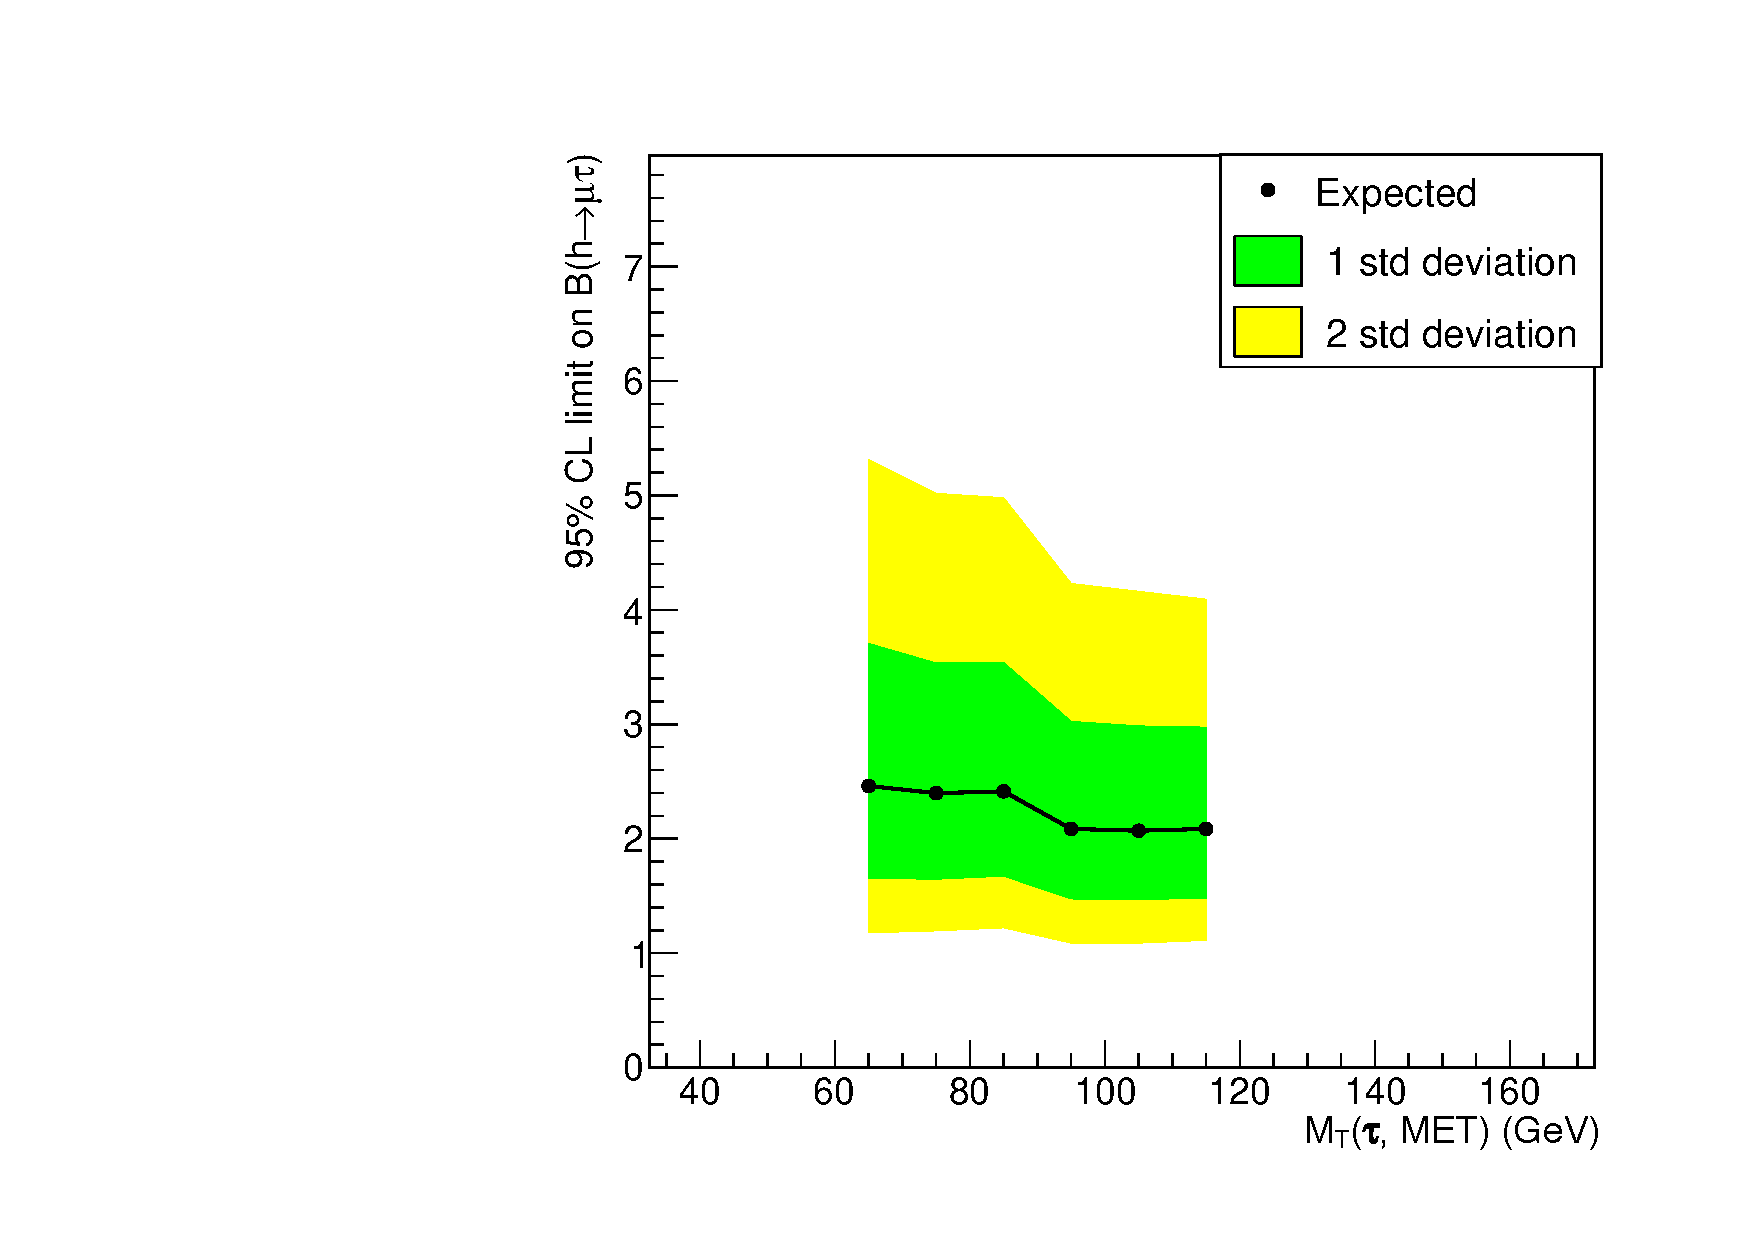
\includegraphics[width=0.4\textwidth]{chapter6/Tuning/boosttMtToPfMet_type1.pdf}}\\
     \subfigure[2 jets, gg-enriched]{ 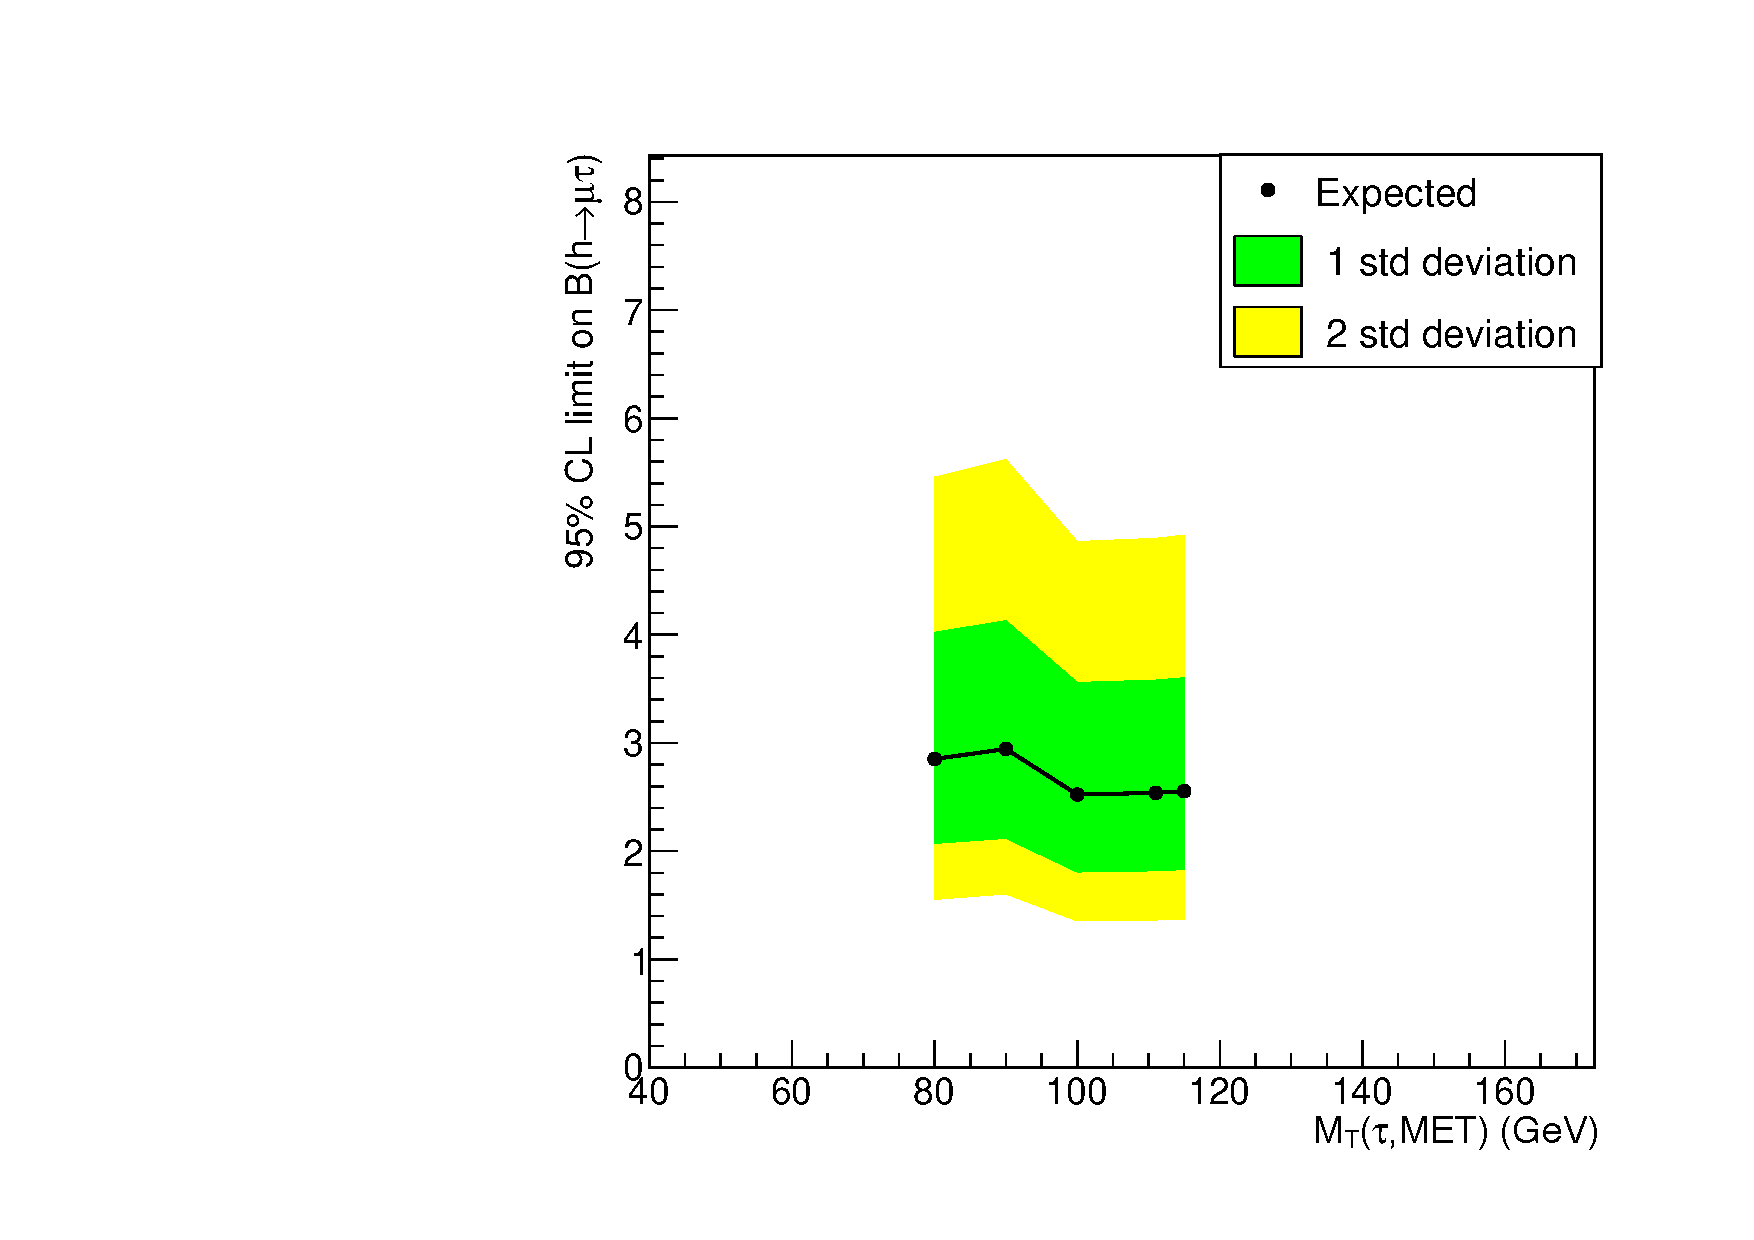
\includegraphics[width=0.4\textwidth]{chapter6/Tuning/vbf_ggtMtToPfMet_type1.pdf}}
     \subfigure[2 jets, VBF-enriched]{ 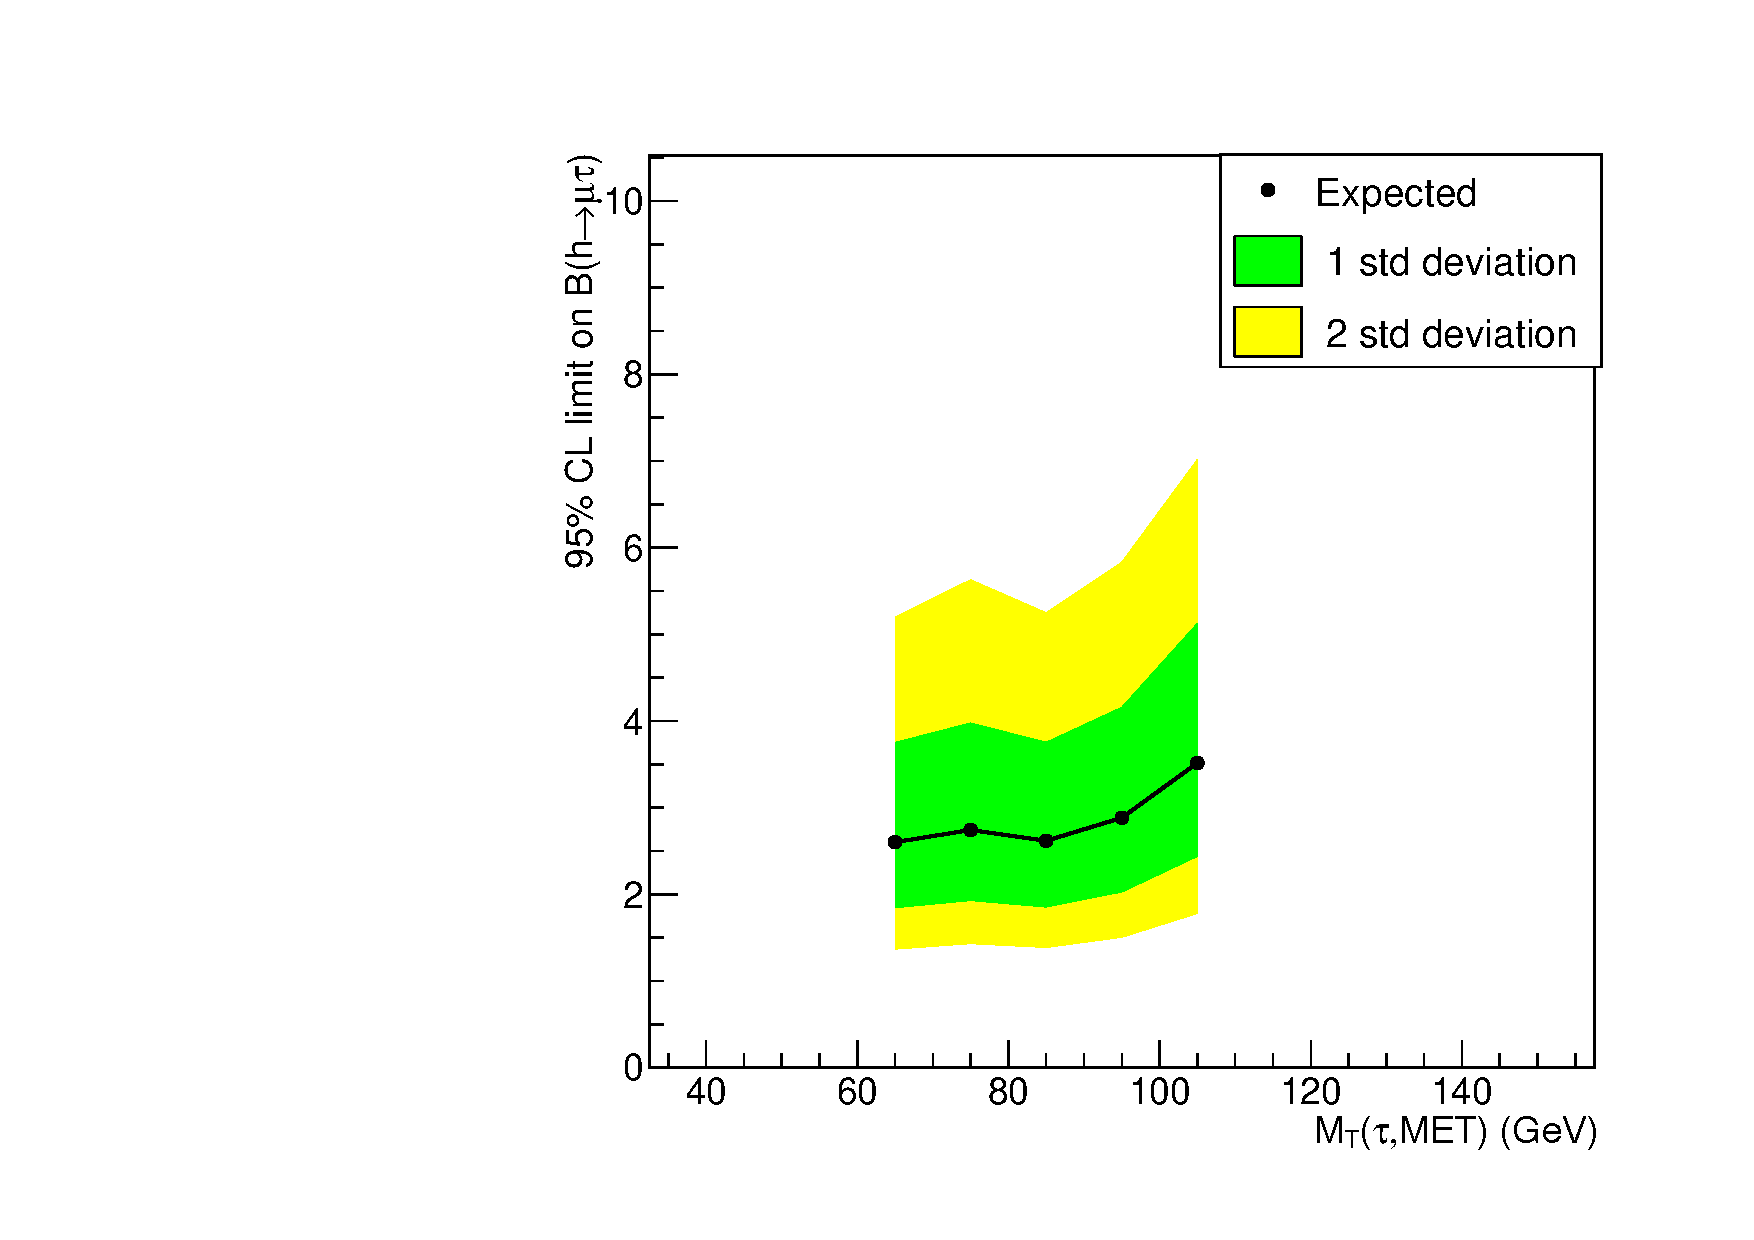
\includegraphics[width=0.4\textwidth]{chapter6/Tuning/vbf_vbftMtToPfMet_type1.pdf}}
     \caption{Expected limits based on an Asimov dataset as a function of $M_T(\tau, MET)$ for the different categories.}
     \label{fig:optMT}
\end{figure}

\begin{figure}[!htbp]
\centering
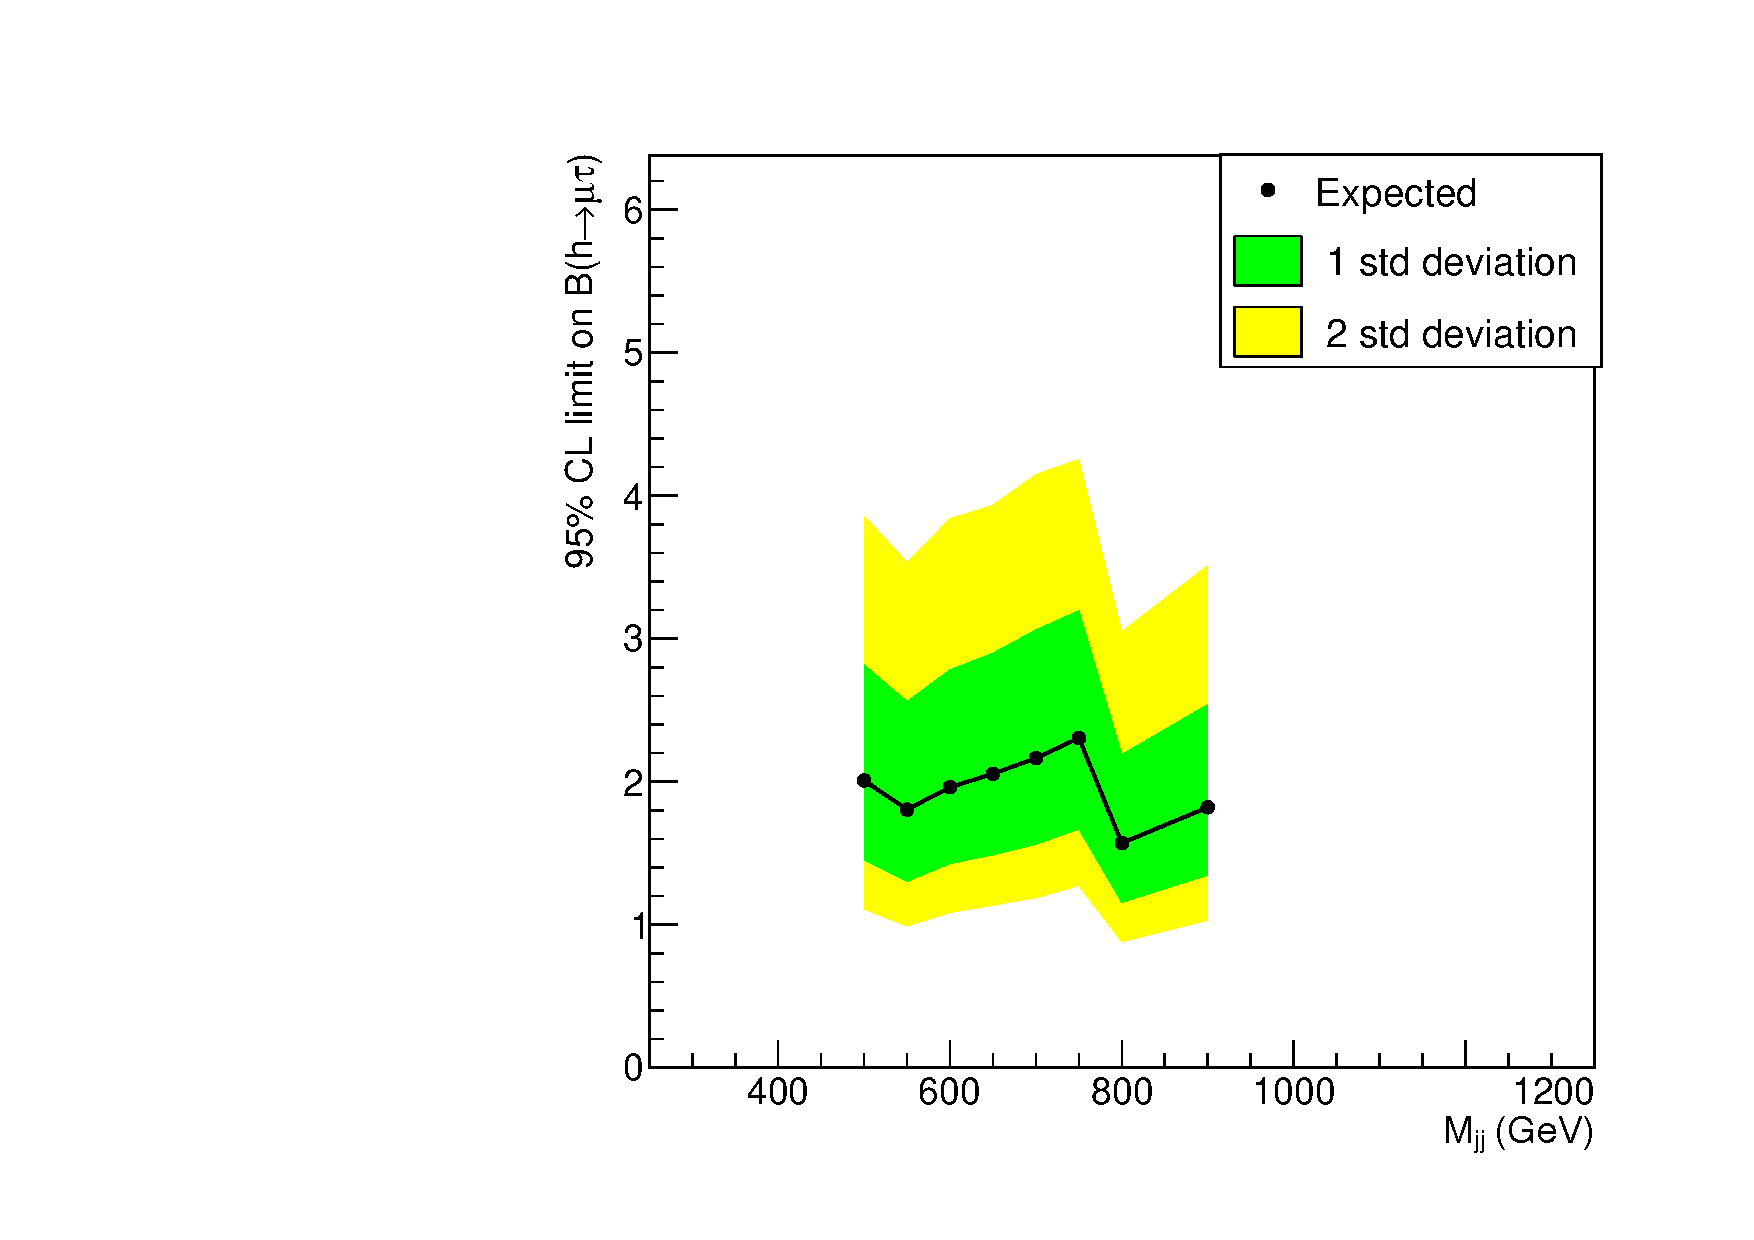
\includegraphics[width=0.4\textwidth]{chapter6/Tuning/vbf_vbfvbfMass.pdf}
\caption{Expected limits based on an Asimov dataset as a function of $M_{jj}$ for the 2 jet categories.}
\label{fig:optVBFmass}
\end{figure}




\subsection{Multivariate analysis}
A Boost decision trees(BDT) method is chosen as the multivariate analysis method used in  $H\rightarrow\mu\tau_h$ search. It provides greater sensitivity compared with the cut-based analysis. BDT method takes in two set of datasets, signal and background and a selected set of input variables. The input variables are the ones that show distinguishing power between signal and background.  The training output is a weight file, which contains a list of weights to indicate in percentage how likely an event is signal like with a give set of input variable values from that event. A more detail description of the BDT method is available in section \ref{BDTchaper}.  In this analysis, signal and background events are required to pass the lose selection criteria. All of the categories are combined. The signal events from gluon gluon fusion and vector boson fusion higgs production mode are mix by the weight with their respective production cross section. The background sample used in the training is fake background in the like sign region(Region II as in table **),  which is orthogonal to the signal region and avoid double use the data.  The distribution of input variables in the BDT training is the shown in Fig.~\ref{fig:BDTvariable}.

\begin{itemize}
\item Transverse mass between the $\tauh$ and $\ETmiss$, $M_{T}(\tau_{h})m$.
\item Missing transverse energy, $\ETmiss$.
\item Pseudorapidity difference between the muon  and the $\tauh$ candidate, $\Delta\eta(\Pgm, \tauh)$.
\item Azimutal angle between the muon and the $\tauh$, $\Delta\phi(\Pgm,\tauh)$.
\item Azimutal angle between the $\tauh$ and the $\ETmiss$, $\Delta\phi(\tau_h,\ETmiss)$.
\item Collinear mass, $\mcol$.
\item Muon $\pt$.
\item $\tau_h$ $\pt$.
\end{itemize}

\begin{figure}[htpb] \label{fig:BDTvariable}
\begin{center}
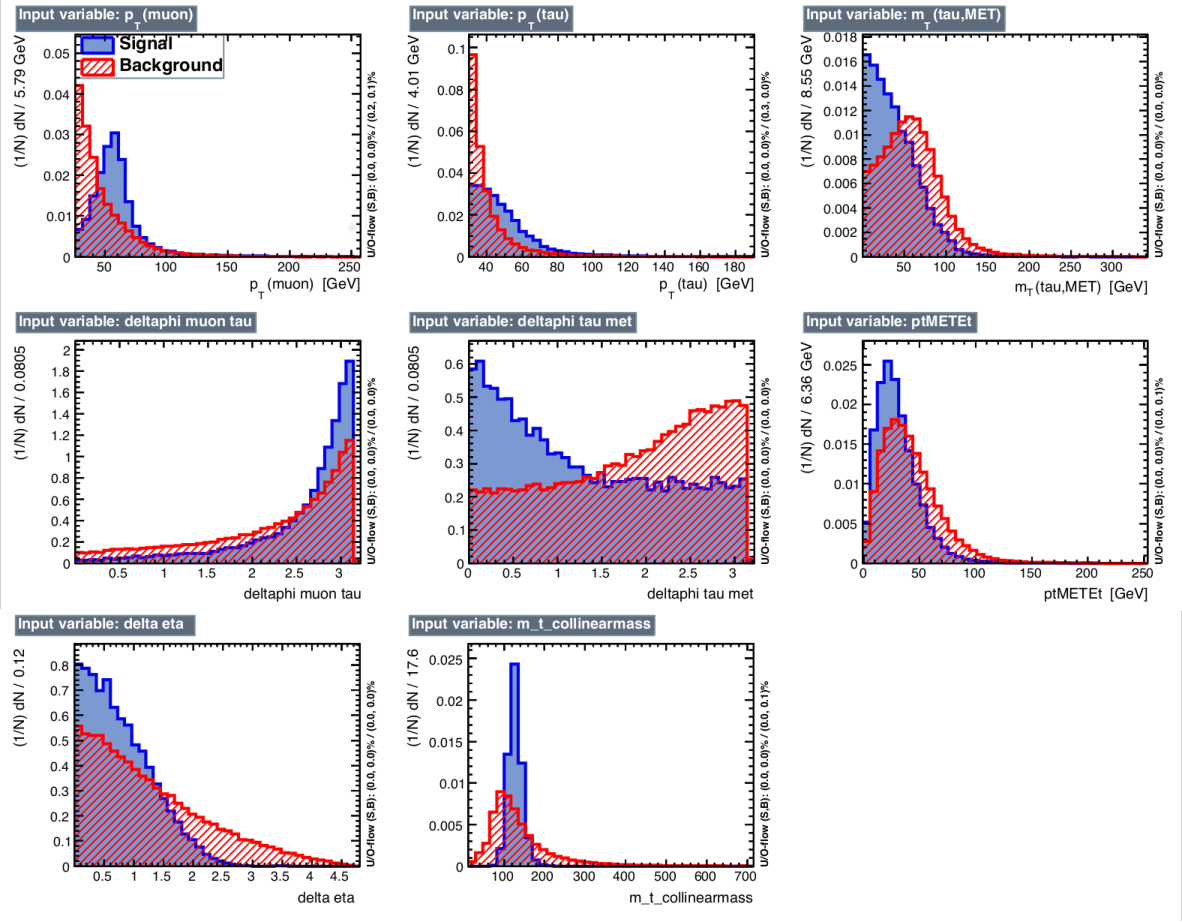
\includegraphics[width=1.\textwidth]{chapter6/BDTvariable.pdf}
\end{center}
\caption{$\Hmuhad$: BDT input variable distributions. Signal distributions are drawn in blue and the background  distributions in red.}
\label{fig:bdtInputHmuh}
\end{figure}










